\section{ОБЩЕТЕХНИЧЕСКИЙ АНАЛИЗ ПРОЕКТИРУЕМОГО УСТРОЙСТВА}
\subsection{Анализ исходных данных}
\par
В курсовой работе рассматривается беспроводной роутер асимметричной
цифровой абонентской линии.  Чтобы кратко сформулировать назначение
данного сетевого устройства достаточно одного слова — маршрутизатор.
Потому что именно задачу маршрутизации, то есть доставки сетевых
пакетов из пользовательской сети в сеть интернет-провайдера решают
такого рода устройства.
\par
Одной из функций маршрутизатора является физическогое соединение
сетей. Маршрутизатор имеет несколько сетевых интерфейсов, подобных
интерфейсам компьютера, к каждому из которых может быть подключена
одна сеть. Маршрутизатор может быть реализован программно на базе
универсального компьютера (например, типовая конфигурация Unix или
Windows включает программный модуль маршрутизатора). Однако чаще
маршрутизаторы реализуются на базе специализированных аппаратных
платформ. В состав программного обеспечения маршрутизатора входят
протокольные модули сетевого уровня ~\cite{NetworksOlifer2016}.

Роутер выполнен в виде платы с распаянными компонентами, в
негерметичном корпусе с перфорацией для обеспечения естественной
вентиляции РЭС. Корпус имеет форму параллелепипида, на задней панели
содержит разъём RJ-45 для подключения к телефонной сети и четыре
разъёма для подключения по стандарту Ethernet, антенну, разъём питания
и тумблер включения.

\begin{figure}[h] %% h means here
  \centering
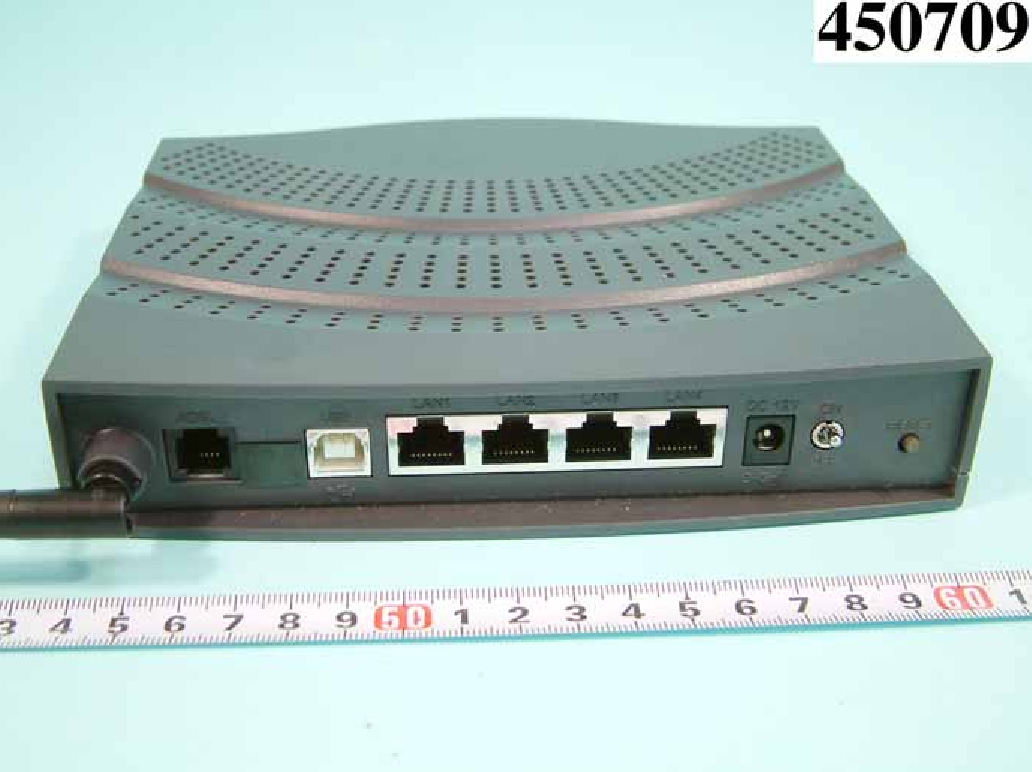
\includegraphics[scale = 0.7]{external_photos-2.png}
\caption{Фотография задней панели роутера ~\cite{EXTERNAL_PHOTOS}.}

\end{figure}

Поскольку в курсовой работе будет производиться расчёт тепловых
режимов будет также важно учитывать климатические факторы внешней
среды, то какие условия эксплутации при этом должны быть соблюдены
регламентирует соответсвующий стандарт — ГОСТ 15150-69
~\cite{GOST_15150-69}.

Настоящий стандарт должен применяться при проектировании изделий.  В
частности, он должен применяться при состалвении технических заданий
на разработку или модернизацию изделий, а также при разработке
государственных стандартов и технических условий, устанавливающих
требования в части воздействия климатических факторов внешней среды
для группы изделий, а при отсуствии указанных групповых документов —
для отдельных видов изделий ~\cite{GOST_15150-69}.

Для конкретных типов или групп изделий виды воздействующих
климатических факторов и их номинальные значения устанавливаются в
зависимости от условий эксплуатации изделий в соответвующих
технических заданих, стандартах и технических условиях ~\cite{GOST_15150-69}.

Так как в данном случае роутер предоставляет доступ в интернет в
пределах одного дома, квартиры или небольшого офиса. Можно говорить, что роутер соответствует категории УХЛ 4.2 ГОСТ15150-69.

Характеристика данной категории следующая:\\
Для эксплуатации в помещниях (объемах) с искуственно регулируемыми
климатическими условиями, например в закрытых отапливаемых или
охлаждаемых и вентелируемых производственных и других, в том числе
хорошо вентилиуруемых подземных помещниях (отсуствие воздействия
прямого соленчного излучения, атмосферных осадков, ветра, песка и пыли
наружного воздуха; отсутвие или существенное уменьшение воздействия
рассеяного солнечного излучения и конденсации влаги). Для эксплуатации
в лабораторных, капитальных и других подобного типа помещениях ~\cite{GOST_15150-69}.

Соответствие условий работы роутера ассиметричной цифровой абонетской
линии данному ГОСТ важно по той причине, что климатические условия
регламентиуремые ГОСТ влияют на внешние тепловые воздействия на РЭС.
В зависимости от них также может быть выбран корпус определённого
типа.

\subsection{Описание принципа работы анализируемого устройства}


Рассмотренной устройство — специализированная аппартная платформа,
реализующего фукнции маршрутизатора в сетевой топологии.  Чтобы ещё
больше конкретизировать назначение устройства необходимо упомянуть в
каком сегменте сети оно осуществляет свою работу.


Локальная сеть (LAN, Local Area Network) — частная сеть,
функционирующая в отдельном здании и на прилегающей территории
(это может быть дом, офис или завод). LAN широко применяется для соединения персоналтьны компьютеров и бытовой электроники, позволяя совместно
использовать различные ресурсы (например, принтеры) и обмениваться
информацией ~\cite{NetworksTanenbaum2023}.

На сегодняшний день беспроводные LAN применяются
повсеместно. Изначально они были популярны в жилых помещениях, старых
офисных зданиях, кафе и других местах, где прокладка кабелей обошлась
бы слишком дорого. В подобных система компьютеры обмениваются
информацией с помощью встроенного радиомодема и антенны. Чаще всего
компьютер обращается к специальному устройству, которой называется
точкой доступа (AP, Access Point), беспроводным маршрутизатором
(wireless router) или базовой станцией (base station). Это устройство
осуществляет передачу пакетов данных между беспроводными компьютерами,
а также между компьютером и интернетом. Точка доступа напоминает
популярного ребенка в школе, поскольку все хотят с ней «поговорить»
~\cite{NetworksTanenbaum2023}.

Одним из самых популярных стандартов беспроводных LAN является IEEE
802.11, более известный как wi-fi ~\cite{NetworksTanenbaum2023}.

И именно этому стандарту следует рассматриваемое устройство.

Вместо дорогостоящих лицензируемых частот системы 802.11 работают на
нелицензируемых полосах частот, например ISM («Industrial, Scientific,
and Medical» — «промышленные, научные и медицинские») устанавливаемых
МСЭ-R (например 902-928 МГц, 2,4-2,5 ГГц, 5,725-5,825 ГГц).  Этот
диапазон частот разрешено использовать любым устройствам, но мощность
их излучения должна быть ограничена, чтобы различные устройства не
мешали друг другу. Конечно, из-за этого 802.11-передатчики иногда
начинают конкурировать за частоты с беспроводными телефонами,
системами дистанционного открывания дверей гаража и микроволновками.
Так что до тех пор, пока пользователям не понадобиться позвонить
гаражным дверям, важно все настроить
правильно ~\cite{NetworksTanenbaum2023}.

Таким образом рассмотренное устройства это РЭС основная задача
которого — это прием, модуляция, обработка и передача сигнала другим
устройствам и аппаратуре. При этом, поскольку устройство производит не
только физическую передачу данных, но и коммутацию сетевых пакетов,
оказываются нужными некоторые вычислительные ресурсы.
Следовательно для того чтобы осуществлять вычисления устройство будет
оснащенно микропроцессором.

\subsection{Анализ элементной базы устройства}

Используя блок схему рассмотрим элементную базу
маршрутизатора.


\begin{figure}[h] %% h means here
  \centering
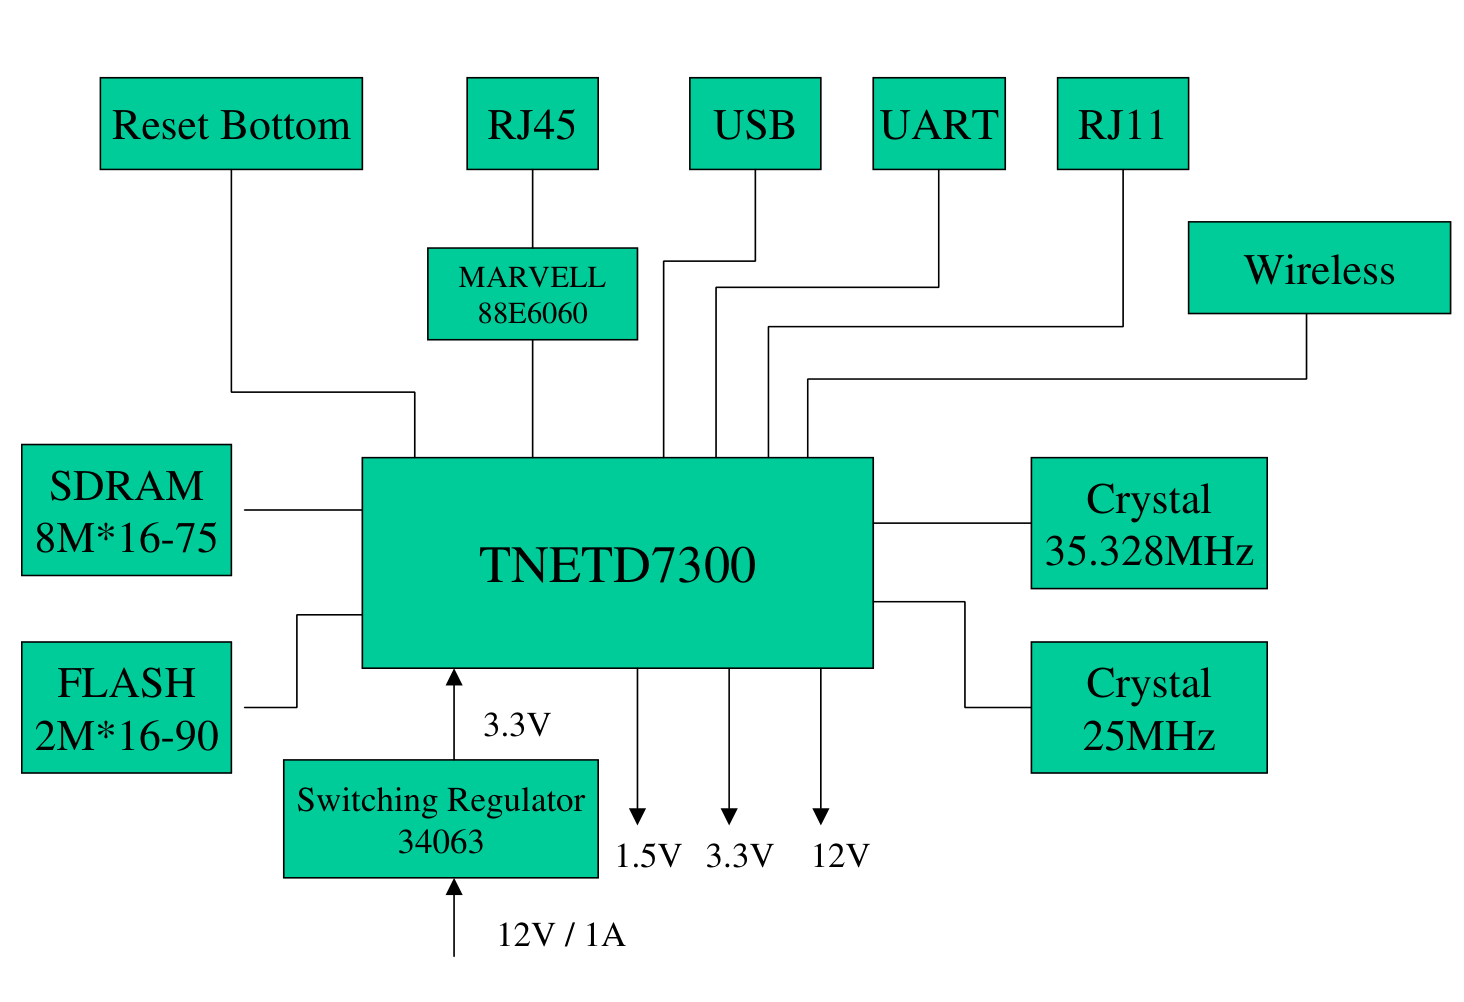
\includegraphics[scale = 0.7]{block_diagram-0.png}
\caption{Блок схема устройства маршрутизатора ASW800ADSL ~\cite{BLOCK_DIAGRAM}.}
\end{figure}
 
Как видно из блок схемы первостепенным и самым важным модулем данной
РЭС явяляется чип TNETD7300, он расположен в цетрне блок схемы. С ним
соеденены несколько интерфейсов и остальные модули.

Из того как расположен этот модуль на блоксхеме можно сделать вывод,
что в этой части РЭС будет рассеиваться больше всего мощности.

Различают внтуренние и внешние тепловые воздействия на РЭА.
Внутренние тепловые воздействия на РЭА в основном зависят от мощности
рассеиваемой её элементами ~\cite{Rotkop1976}.

Энергетический коэффициент полезного действия радиоэлементов, как
правило, невелик, и значительная доля энергии питания превращается в
тепловую энергию с сопутствующим перегревом элементов и аппаратуры
~\cite{Rotkop1976}.

Насыщение современных технических устройств РЭА различного назначения
заставляет конструкторов уменьшать ее габариты и увеличивать удельные
мощности рассеивания, т.е. мощности, приходящиеся на единицу
поверхности или объема РЭА. Одним из основных направлений в
конструировании РЭА стала комплексная микроминиатюризация, что
приводит к ещё большему увелечению удельной мощности рассеивания
~\cite{Rotkop1976}.

%% \pagebreak
Рассмотрим схему электрическую принципиальную на которой изображён чип
TNETD7300.

\begin{figure}[hb]
  \centering
  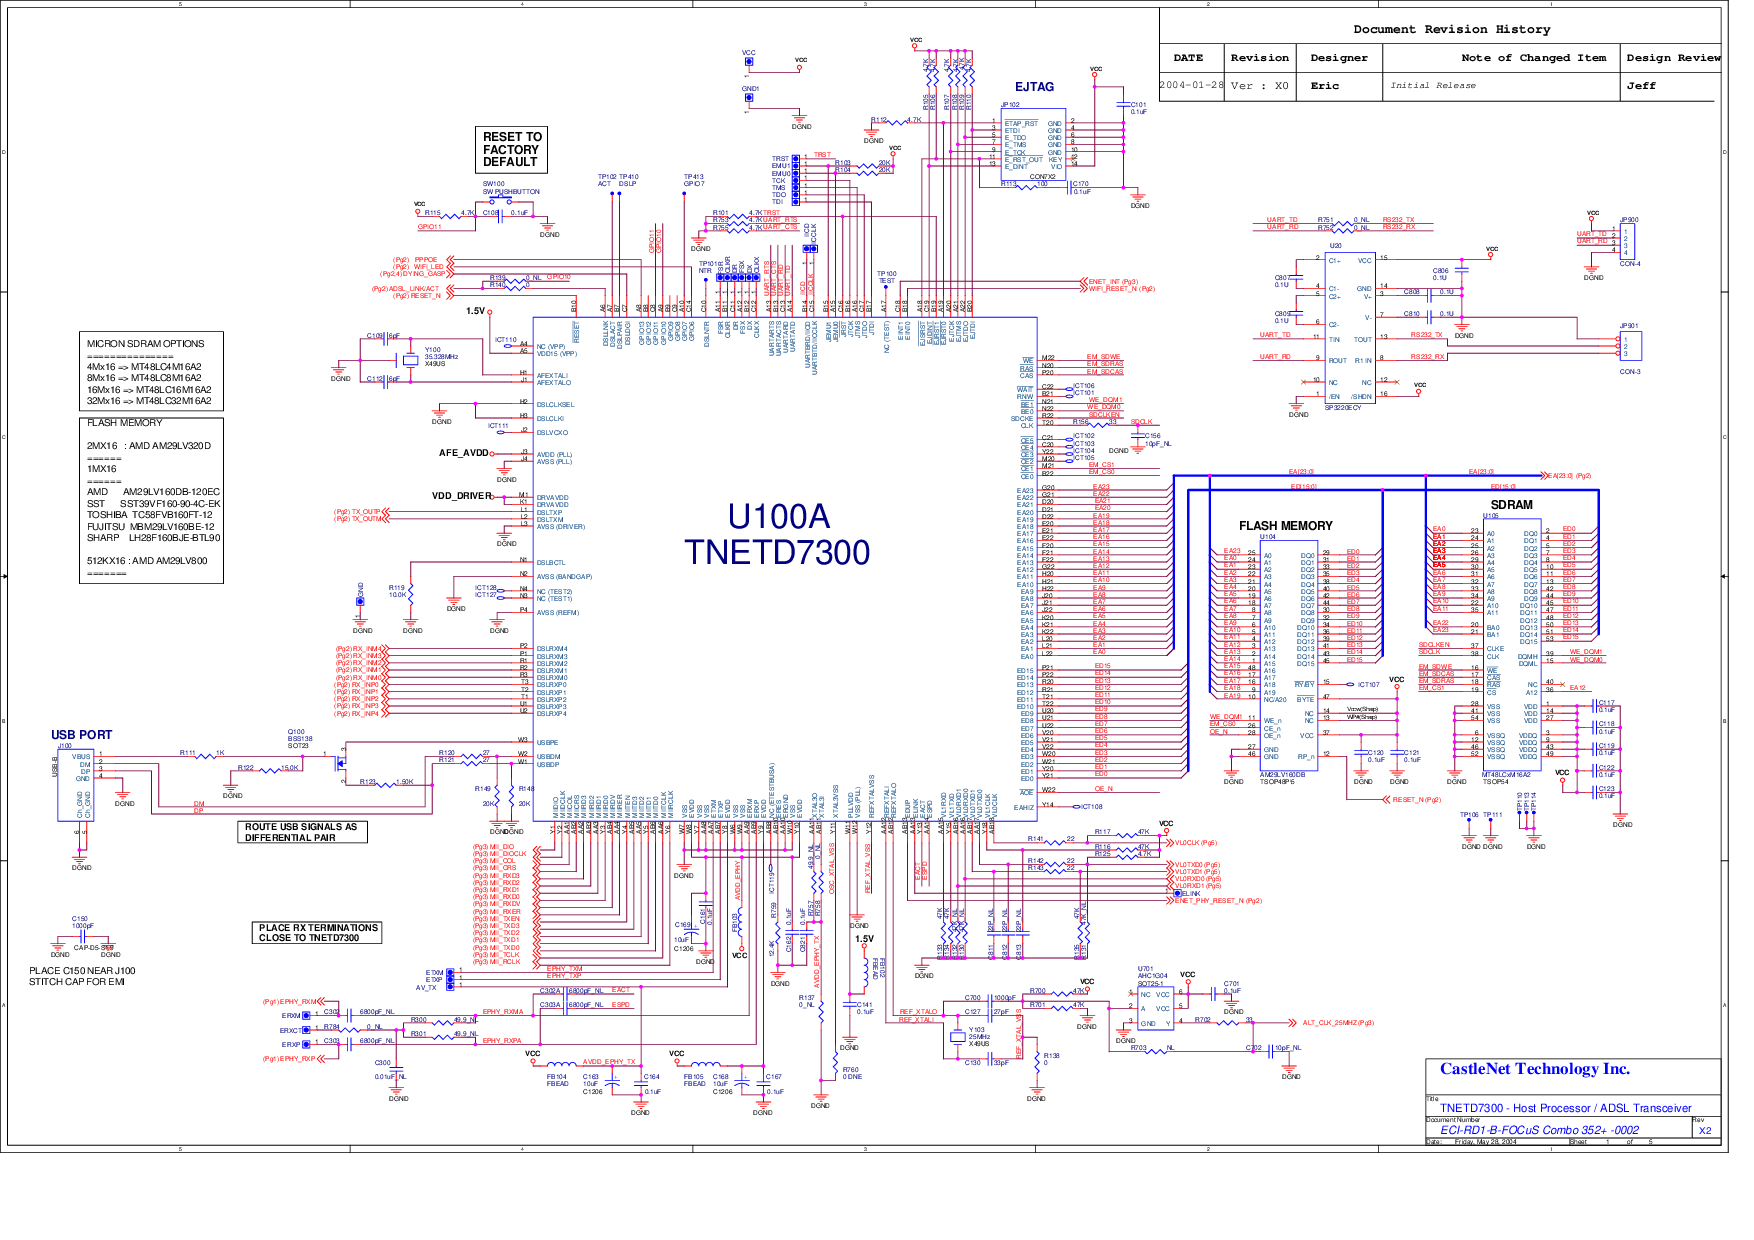
\includegraphics[scale = 0.25]{schematics-1.png}
  \caption{Схема электрическая принципиальная
    маршрутизатора ASW800ADSL ~\cite{SCHEMATICS}.}
\end{figure}

На схеме чип TNETD7300 подписан не иначе как \textit{«Host Proccessor»}.
Из этого можно сделать вывод, что, уже упомянутым в предыдущем
параграфе, микропроцессором и будет являться этот чип.  На схеме
электрической принципиальной микропроцессор выглядит как квадрат к
которому подведены другие компоненты. Такой способ изображения вызван
тем, что для того чтобы показать все элементы из которых состоит
процессор требуется отдельная большая подсхема, которая в свою очередь
была бы разделена на несколько других подсхем соответствующих
отдельным частями процессора, таким как арифметико логическое
устройство, блок управления памятью и другие. Это ещё раз подтверждает
вывод о том, что данное устройство рассеивает больше всего мощности, а
значит и требует наибольшего охлаждения.

\subsection{Выбор и обоснование системы охлаждения}

Защита от тепловых воздействий это одна из важных задач решаемых в обеспечении недёжности РЭС.

Защита РЭА от тепловых воздействий осуществляется при помощи ряда
мероприйтий. Одним из основных является использование систем
обеспечения теплового режима РЭА (СОТР). СОТР обычно предназначена для
поддержания заданного в технических условиях (ТУ) диапазона температур
на элементах РЭА, чтобы обеспечить ее надежность при определенных
тепловых воздействиях и других специальных требованиях ~\cite{Rotkop1976}.

В радиоэлектронных комплексах СОТР, как правило, являются сложными
системами, состоящими из многих элементов, коммуникациий и несущих
конструкий. В некоторых случаях регулирование температуры в РЭА может
быть достигнуто за счет простейших конструктивных решений,
осущствляющих теплопередачу между элементами РЭА, элементами несущей
конструкции и окружающей средой. Тогда нет смысла рассматривать СОТР
как отдельное изделие и мы будем пользоваться терминами «методы (или
спосбы) охлаждения РЭА». Этими же терминами будем пользоваться и при
исследовании температурного поля элементов РЭА, в результате действия
некоторых гипотетических СОТР, когда конкретная конструкция СОТР не
рассматривается ~\cite{Rotkop1976}.

Для выбора и обоснование системы охлаждения важно иметь представление
о тепловом режиме РЭС.  Тепловой режим есть совокупность значений
температур в различных точках всей РЭС, её корпуса и СОТР.

Тепловой режим РЭА характеризуется, прежде всего, двумя факторами:
электрическим режимом работы и условиями эксплуатации ~\cite{Rotkop1976}.

Электрический режим работы РЭА в данном случае интересует нас только в
связи с измененением внутренних тепловых воздействий во времени и
пространстве и задается обычно в виде графиков зависимости
рассеиваемой мощности от времени для различных узлов РЭА~\cite{Rotkop1976}.

%% Сюда вставить график где Q = x = const; t = y


По приведённому графику видно, что режим работы данного РЭС —
длительный. То есть устройство работает в течении достаточно большого
периода времени рассеивая постоянную по величине мощность.

Такой электрический режим не позволит использовать радиаторы в виде
так назывымых тепловых аккумуляторов.

Данные касаемо условий эксплуатации были приведены ранее и
соответсвуют условиям категории УХЛ 4.2 указанным в ГОСТ
~\cite{GOST_15150-69}.

Понятию «достаточно большой промежуток времени» в контесте охлаждения
РЭС соответствует такой промежуток времени, за который полностью
устанавливается тепловой режим этого РЭС.

Учитывая тип и состояние теплоносителя, также причину, вызвавшую его
движение, способы охлаждения РЭА можно разделить на следующие основные
классы: газовое (воздушное), жидкостное, испарительное, а также
естественное и принудительное ~\cite{Rotkop1976}.

Здесь некоторый способ охлаждения может относиться сразу к двум
классам: по агрегатному состоянию теплоносителя и тому принудительно
ли осуществляется охлаждение.

В данном случае создатели устройства выбрали класс естественного
воздушного охлаждения.

Естественное воздушное охлаждение РЭА является наиболее простым,
надежным и дешевым способом охлаждения и осущствляется без затрыты
дополнительной энергии. Однако интенсивность такого охлаждения
невелика, поэтому использование этого способа возможно при небольших
удельных мощностях мощностяхрассеивания (мощностях, рассеиваемых
единицей поверхности или объема), т.е. в РЭА, работающей в облегченном
тепловом режиме. При естественном воздушном охлаждении конвективный
теплообмен осущствляется за счет энергии, рассеиваемой элементами РЭА ~\cite{Rotkop1976}.

Для подтверждения предположений касательно класса и схемы охлаждения
РЭС обратимся к его внутренниму устройству. Для этого рассмотрим
фотографию печатной платы со снятой крышкой корпуса.

\begin{figure}[hb]
  \centering
  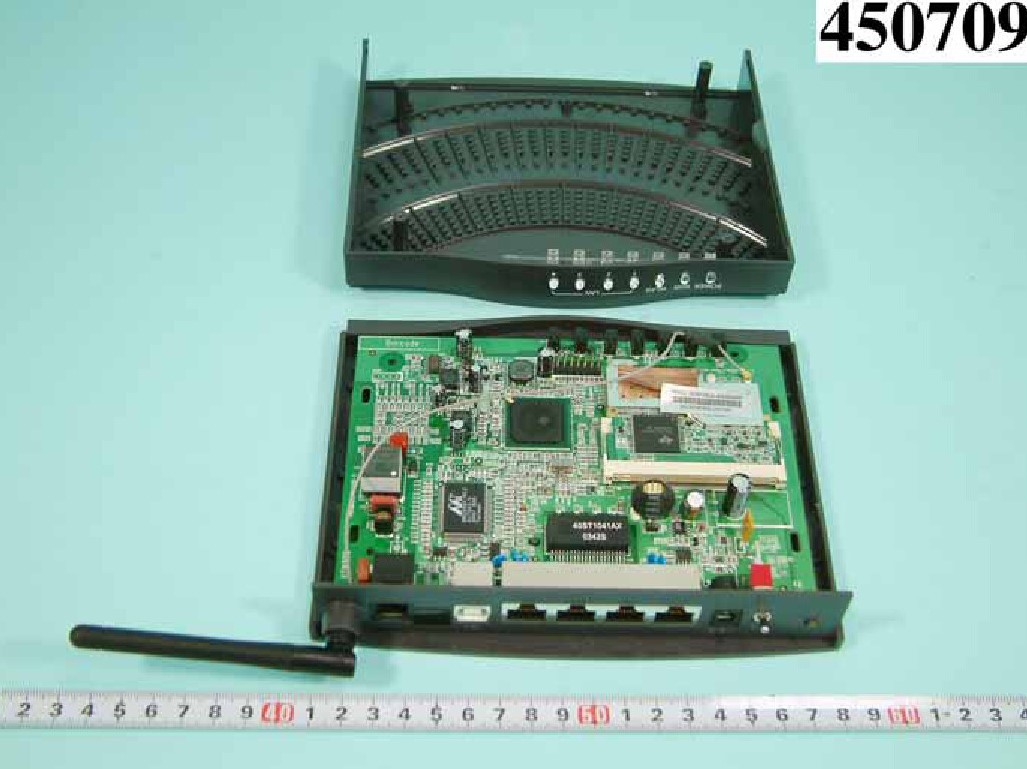
\includegraphics[scale = 0.65]{internal-0.jpg}
  \caption{Корпус РЭС со снятой крышкой ~\cite{INTERNAL_PHOTOS}.}
\end{figure}

На приведённой фотографии видно отсуствие прикреплённого к чипу
радиатора или вентилятора продувающего корпус.

Также на фотографии заметна перфорация корпуса. Притом заметно
значительное количество отверстий перфорации.

Естественное воздушное охлаждение РЭА с перфорированным кожухом
позволяет обеспечить тепловой режим при более высоких удельных
мощностях рассеивания, чем при герметичном кожухе ~\cite{Rotkop1976}.

Таким образом можно подытожить: класс охлаждения РЭС — естественное
воздушное охлаждение, а схема охлаждения — охлаждение с
перфорированным корпусом. Данный выбор системы охлаждения обусловлен
необходимостью тратить меньше энергии на охлаждение устройства, чем на
им производимые вычисления. Такой подход также можно обосновать
простотой получившийся конструкции. СОТР как таковая отсуствует,
потому можно говорить только о методах охлаждения, а не о конструкции
конкретной СОТР.

\newpage
%% Это видимо конец главы.